\documentclass{beamer}
\usepackage[utf8]{inputenc}

\usetheme{Madrid}
\usecolortheme{default}
\usepackage{amsmath,amssymb,amsfonts,amsthm}
\usepackage{txfonts}
\usepackage{tkz-euclide}
\usepackage{listings}
\usepackage{adjustbox}
\usepackage{array}
\usepackage{tabularx}
\usepackage{gvv}
\usepackage{lmodern}
\usepackage{circuitikz}
\usepackage{tikz}
\usepackage{graphicx}

\setbeamertemplate{page number in head/foot}[totalframenumber]

\usepackage{tcolorbox}
\tcbuselibrary{minted,breakable,xparse,skins}

\definecolor{bg}{gray}{0.95}
\DeclareTCBListing{mintedbox}{O{}m!O{}}{%
  breakable=true,
  listing engine=minted,
  listing only,
  minted language=#2,
  minted style=default,
  minted options={%
    linenos,
    gobble=0,
    breaklines=true,
    breakafter=,,
    fontsize=\small,
    numbersep=8pt,
    #1},
  boxsep=0pt,
  left skip=0pt,
  right skip=0pt,
  left=25pt,
  right=0pt,
  top=3pt,
  bottom=3pt,
  arc=5pt,
  leftrule=0pt,
  rightrule=0pt,
  bottomrule=2pt,
  toprule=2pt,
  colback=bg,
  colframe=orange!70,
  enhanced,
  overlay={%
    \begin{tcbclipinterior}
    \fill[orange!20!white] (frame.south west) rectangle ([xshift=20pt]frame.north west);
    \end{tcbclipinterior}},
  #3,
}

% Code style
\lstset{
    language=C,
    basicstyle=\ttfamily\small,
    keywordstyle=\color{blue},
    stringstyle=\color{orange},
    commentstyle=\color{green!60!black},
    numbers=left,
    numberstyle=\tiny\color{gray},
    breaklines=true,
    showstringspaces=false,
}

%------------------------------------------------------------
% Title info
\title %optional
{4.2.16}
\date{September 6, 2025}
\author % (optional)
{Bhargav - EE25BTECH11013}

\begin{document}

\frame{\titlepage}

\begin{frame}{Question}
Find the direction and normal vector for the line 
\begin{align}
    2 + 3y = 7x
\end{align}
\end{frame}

\begin{frame}{Theoretical Solution}
The line can be written as
\begin{align}
    7x - 3y = 2
\end{align}
Let
\begin{align}
    \vec{x} = \myvec{x \\ y}, \quad
    \vec{n^T} = \myvec{7 & -3}, \quad
    c = 2
\end{align}
Thus, the line equation is
\begin{align}
    \vec{n^T}\vec{x} = c
\end{align}
where $\vec{n}$ is the normal vector.
\end{frame}

\begin{frame}{Direction Vector}
The direction vector of the line can be found by observing the normal vector.
\begin{align}
\vec{m} = \myvec{3 \\ 7}
\end{align}


This is true because if the director vector is represented as 
\begin{align}
\vec{m}  = \myvec{1 \\ m}    
\end{align}
then the normal vector can be represented as 
\begin{align}
\vec{n} = \myvec{-m \\ 1}
\end{align}
\end{frame}

\begin{frame}{Verification}
This can be verified by the following equation:
\begin{align}
\vec{n^T}\vec{m} = 0
\end{align}

\begin{align}
\myvec{7 & -3}\myvec{3 \\ 7} = 0
\end{align}\\    
\end{frame}

\begin{frame}{Final Answer}
\begin{enumerate}
    \item Normal vector: $\vec{n} = \myvec{7 \\ -3}$
    \item Direction vector: $\vec{m} = \myvec{3 \\ 7}$
\end{enumerate}
\end{frame}

\begin{frame}[fragile]
    \frametitle{C Code }

    \begin{lstlisting}

#include <stdio.h>
int dot_product(int a[2], int b[2]) {
    return a[0]*b[0] + a[1]*b[1];
}
int is_orthogonal(int a[2], int b[2]) {
    return dot_product(a, b) == 0;
}
double line_equation(double x) {
    return (7.0*x - 2.0)/3.0;
}


    \end{lstlisting}
\end{frame}

\begin{frame}[fragile]
    \frametitle{Python + C Code }

    \begin{lstlisting}

import ctypes
import numpy as np
import matplotlib.pyplot as plt
lib = ctypes.CDLL("./libcode.so")
lib.dot_product.argtypes = [ctypes.POINTER(ctypes.c_int), ctypes.POINTER(ctypes.c_int)]
lib.dot_product.restype = ctypes.c_int
lib.is_orthogonal.argtypes = [ctypes.POINTER(ctypes.c_int), ctypes.POINTER(ctypes.c_int)]
lib.is_orthogonal.restype = ctypes.c_int
lib.line_equation.argtypes = [ctypes.c_double]
lib.line_equation.restype = ctypes.c_double
normal_vector = (ctypes.c_int * 2)(7, -3)
direction_vector = (ctypes.c_int * 2)(3, 7)
vector_origin = np.array([2, 4])
dp = lib.dot_product(normal_vector, direction_vector)
print(f"Dot product of n and m: {dp}")



    \end{lstlisting}
\end{frame}

\begin{frame}[fragile]
    \frametitle{Python + C code}

    \begin{lstlisting}
if lib.is_orthogonal(normal_vector, direction_vector):
    print("The vectors are orthogonal (as expected).")
else:
    print("The vectors are NOT orthogonal.")
x_vals = np.linspace(-5, 7, 100)
y_vals = [lib.line_equation(float(x)) for x in x_vals]
plt.style.use('seaborn-v0_8-whitegrid')
plt.figure(figsize=(8, 8))
plt.plot(x_vals, y_vals, label='Line: 7x - 3y = 2', color='blue', zorder=1)
plt.quiver(vector_origin[0], vector_origin[1],
           direction_vector[0], direction_vector[1],
           angles='xy', scale_units='xy', scale=1,
           color='green', label='Direction Vector', zorder=2)
plt.quiver(vector_origin[0], vector_origin[1],
           normal_vector[0], normal_vector[1],
           angles='xy', scale_units='xy', scale=1,
           color='red', label='Normal Vector', zorder=2)


    \end{lstlisting}
\end{frame}

\begin{frame}[fragile]
    \frametitle{Python + C code}

    \begin{lstlisting}
plt.plot(vector_origin[0], vector_origin[1], 'o', color='purple', markersize=8,
         label='Vector Origin (2, 4)')
plt.title('Line with Direction and Normal Vectors')
plt.xlabel('x-axis')
plt.ylabel('y-axis')
plt.axis('equal')
plt.legend()
plt.grid(True)
plt.xlim(-5, 10)
plt.ylim(-5, 10)
plt.show()



    \end{lstlisting}
\end{frame}

\begin{frame}[fragile]
    \frametitle{Python code}

    \begin{lstlisting}
import numpy as np
import matplotlib.pyplot as plt

normal_vector = np.array([7, -3])

direction_vector = np.array([3, 7])

print(f"Normal Vector (n): {normal_vector}")
print(f"Direction Vector (m): {direction_vector}")

dot_product = np.dot(normal_vector, direction_vector)
print(f"Dot product of n and m: {dot_product}")
if np.isclose(dot_product, 0):
    print("The vectors are orthogonal (as expected).")
else:
    print("The vectors are NOT orthogonal (something is wrong).")

    \end{lstlisting}
\end{frame}

\begin{frame}[fragile]
    \frametitle{Python code}

    \begin{lstlisting}

def line_equation(x):
    return (7 * x - 2) / 3

x_vals = np.linspace(-5, 7, 100)
y_vals = line_equation(x_vals)

vector_origin = np.array([2, 4])

plt.style.use('seaborn-v0_8-whitegrid')
plt.figure(figsize=(8, 8))
plt.plot(x_vals, y_vals, label='Line: 7x - 3y = 2', color='blue', zorder=1)

plt.quiver(vector_origin[0], vector_origin[1],
           direction_vector[0], direction_vector[1],
           angles='xy', scale_units='xy', scale=1,
           color='green', label='Direction Vector', zorder=2)
    \end{lstlisting}
\end{frame}
\begin{frame}[fragile]
    \frametitle{Python code}

    \begin{lstlisting}
plt.quiver(vector_origin[0], vector_origin[1],
           normal_vector[0], normal_vector[1],
           angles='xy', scale_units='xy', scale=1,
           color='red', label='Normal Vector', zorder=2)
plt.plot(vector_origin[0], vector_origin[1], 'o', color='purple', markersize=8, label='Vector Origin (2, 4)')
plt.title('Line with Direction and Normal Vectors')
plt.xlabel('x-axis')
plt.ylabel('y-axis')
plt.axis('equal')
plt.legend()
plt.grid(True)
plt.xlim(-5, 10)
plt.ylim(-5, 10)
plt.savefig("/Users/bhargavkrish/Desktop/BackupMatrix/ee25btech11013/matgeo/4.2.16/figs/Figure_1.png")
plt.show()


    \end{lstlisting}
\end{frame}

\begin{frame}{Plot}
    \centering
    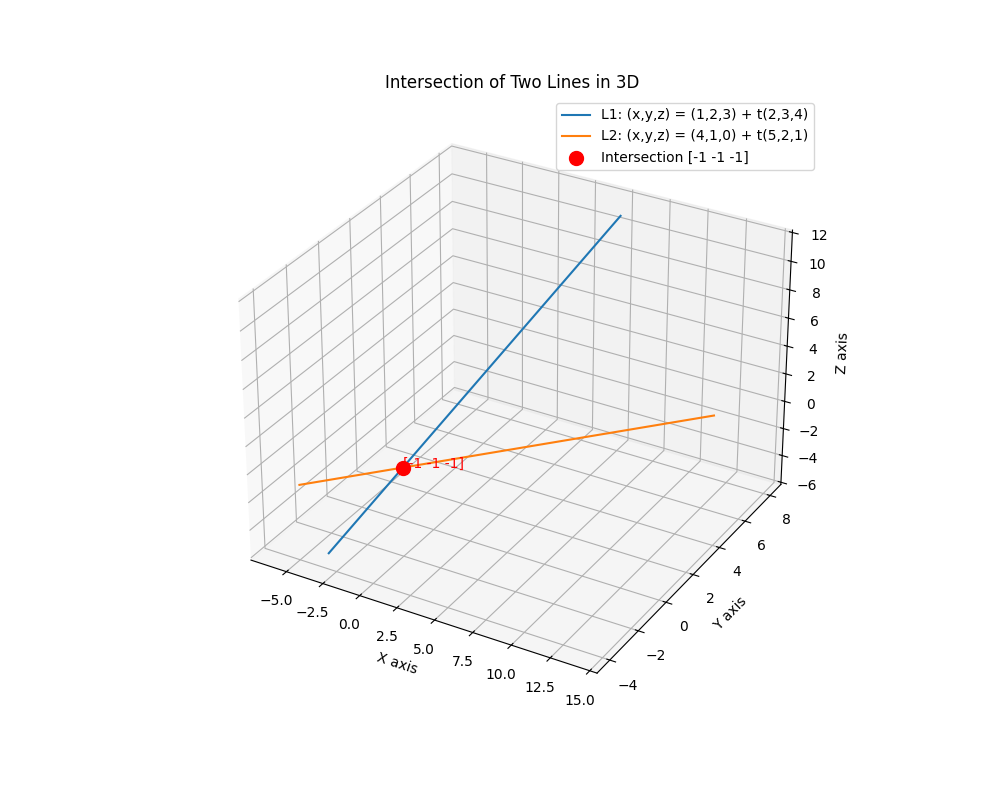
\includegraphics[width=3\columnwidth, height=0.8\textheight, keepaspectratio]{figs/Figure_1.png}     
\end{frame}

\end{document}
